\section{Software de Pesquisa}
\label{section:researchsoftware}

\subsection{Definição}
% definition of Research Software as a separate metaphor of software in research.

O termo \textit{software de pesquisa} foi criado para designar, de modo abrangente, o software \textit{utilizado} durante a pesquisa científica, incluindo o software de terceiros usado para coleta, processamento e análise de dados~\cite{allen_et_al:DM:2017:7146}.
%
%Additional software components (e.g., operating systems, libraries, dependencies, packages, scripts, etc.) that are used for research but were not created during or with a clear research intent should be considered software in research and \textbf{not} Research Software.
%
No contexto de avaliação de qualidade do software de pesquisa,
\cite{gruenpeter_morane_2021_5504016} adotam uma visão mais restrita, e consideram que sistemas operacionais, bibliotecas, dependências, pacotes e \textit{scripts} utilizados na pesquisa científica, mas que não foram criados durante ou com uma intenção de pesquisa clara, são \textit{software usado na pesquisa} mas \textit{não são software de pesquisa}.
% RS should be FAIR! \cite{gruenpeter_morane_2021_5504016}.
% Esta definição erviu para definir o escopo e guiar o trabalho sobre FAIR4RS, identificando os artefatos de software que poderiam ser avaliados segundo tais princípios.
%
No restante deste capítulo, adotaremos a visão de software de pesquisa de~\cite{gruenpeter_morane_2021_5504016}: 

\textit{Software de Pesquisa é o software desenvolvido durante o processo de pesquisa e inclui (mas não está limitado a) código-fonte, algoritmos, \textit{scripts}, fluxos de trabalho computacionais e executáveis.} 

%\subsection{Caracterização}

O \RSw é parte integrante do ecossistema de pesquisa moderno,
sendo amplamente utilizado nas Ciências e Engenharias para gerar resultados que servem como evidência em publicações científicas. 
Em geral, devido à complexidade em desenvolver software e ao conhecimento de domínio especializado necessário, os próprios pesquisadores desenvolvem o \RSw ou estão intimamente envolvidos com o seu desenvolvimento~\cite{carver:icse:2007}.
% Carver survey identifies the steps involved in developing scientific software (i.e. the life cycle, the workflows, technical challenges, and organizational challenges).

Há várias preocupações relacionadas à \textit{natureza} e à \textit{qualidade} do \RS. 
%
Como artefato digital, ele pode assumir muitas formas, por exemplo, um \textit{script} shell bash, com apenas 50 linhas para manipular e filtrar arquivos, um conjunto de \textit{scripts} R de 100 linhas para análise de dados, 10.000 linhas de código Java para software de análise de dívida técnica ou 50.000 linhas de C++ para análise de imagens médicas. 
%Pode ser escrito em linguagens de \textit{script} como Unix shell, Python, R ou MATLAB ou em linguagens de programação como C, C++, Fortran ou Java. 
%
% Ele pode ser hospedado e distribuído de várias maneiras, incluindo repositórios abertos digitais (GitHub, BitBucket, GitLab), projetos como Software Heritage, websites de projetos de pesquisa, pastas FTP, e redes para arquivamento e gerenciamento de artefatos, por exemplo, CRAN (Comprehensive R Archive Network), CPAN (Comprehensive Perl Archive Network), PyPI (Python Package Index), e NPM (Node Package Manager).

%Figura~\ref{fig:mindmap} ... De onde veio mesmo? % (nao sei de onde veio -- joenio)
%\begin{figure}[tbp]
%    \centering
%    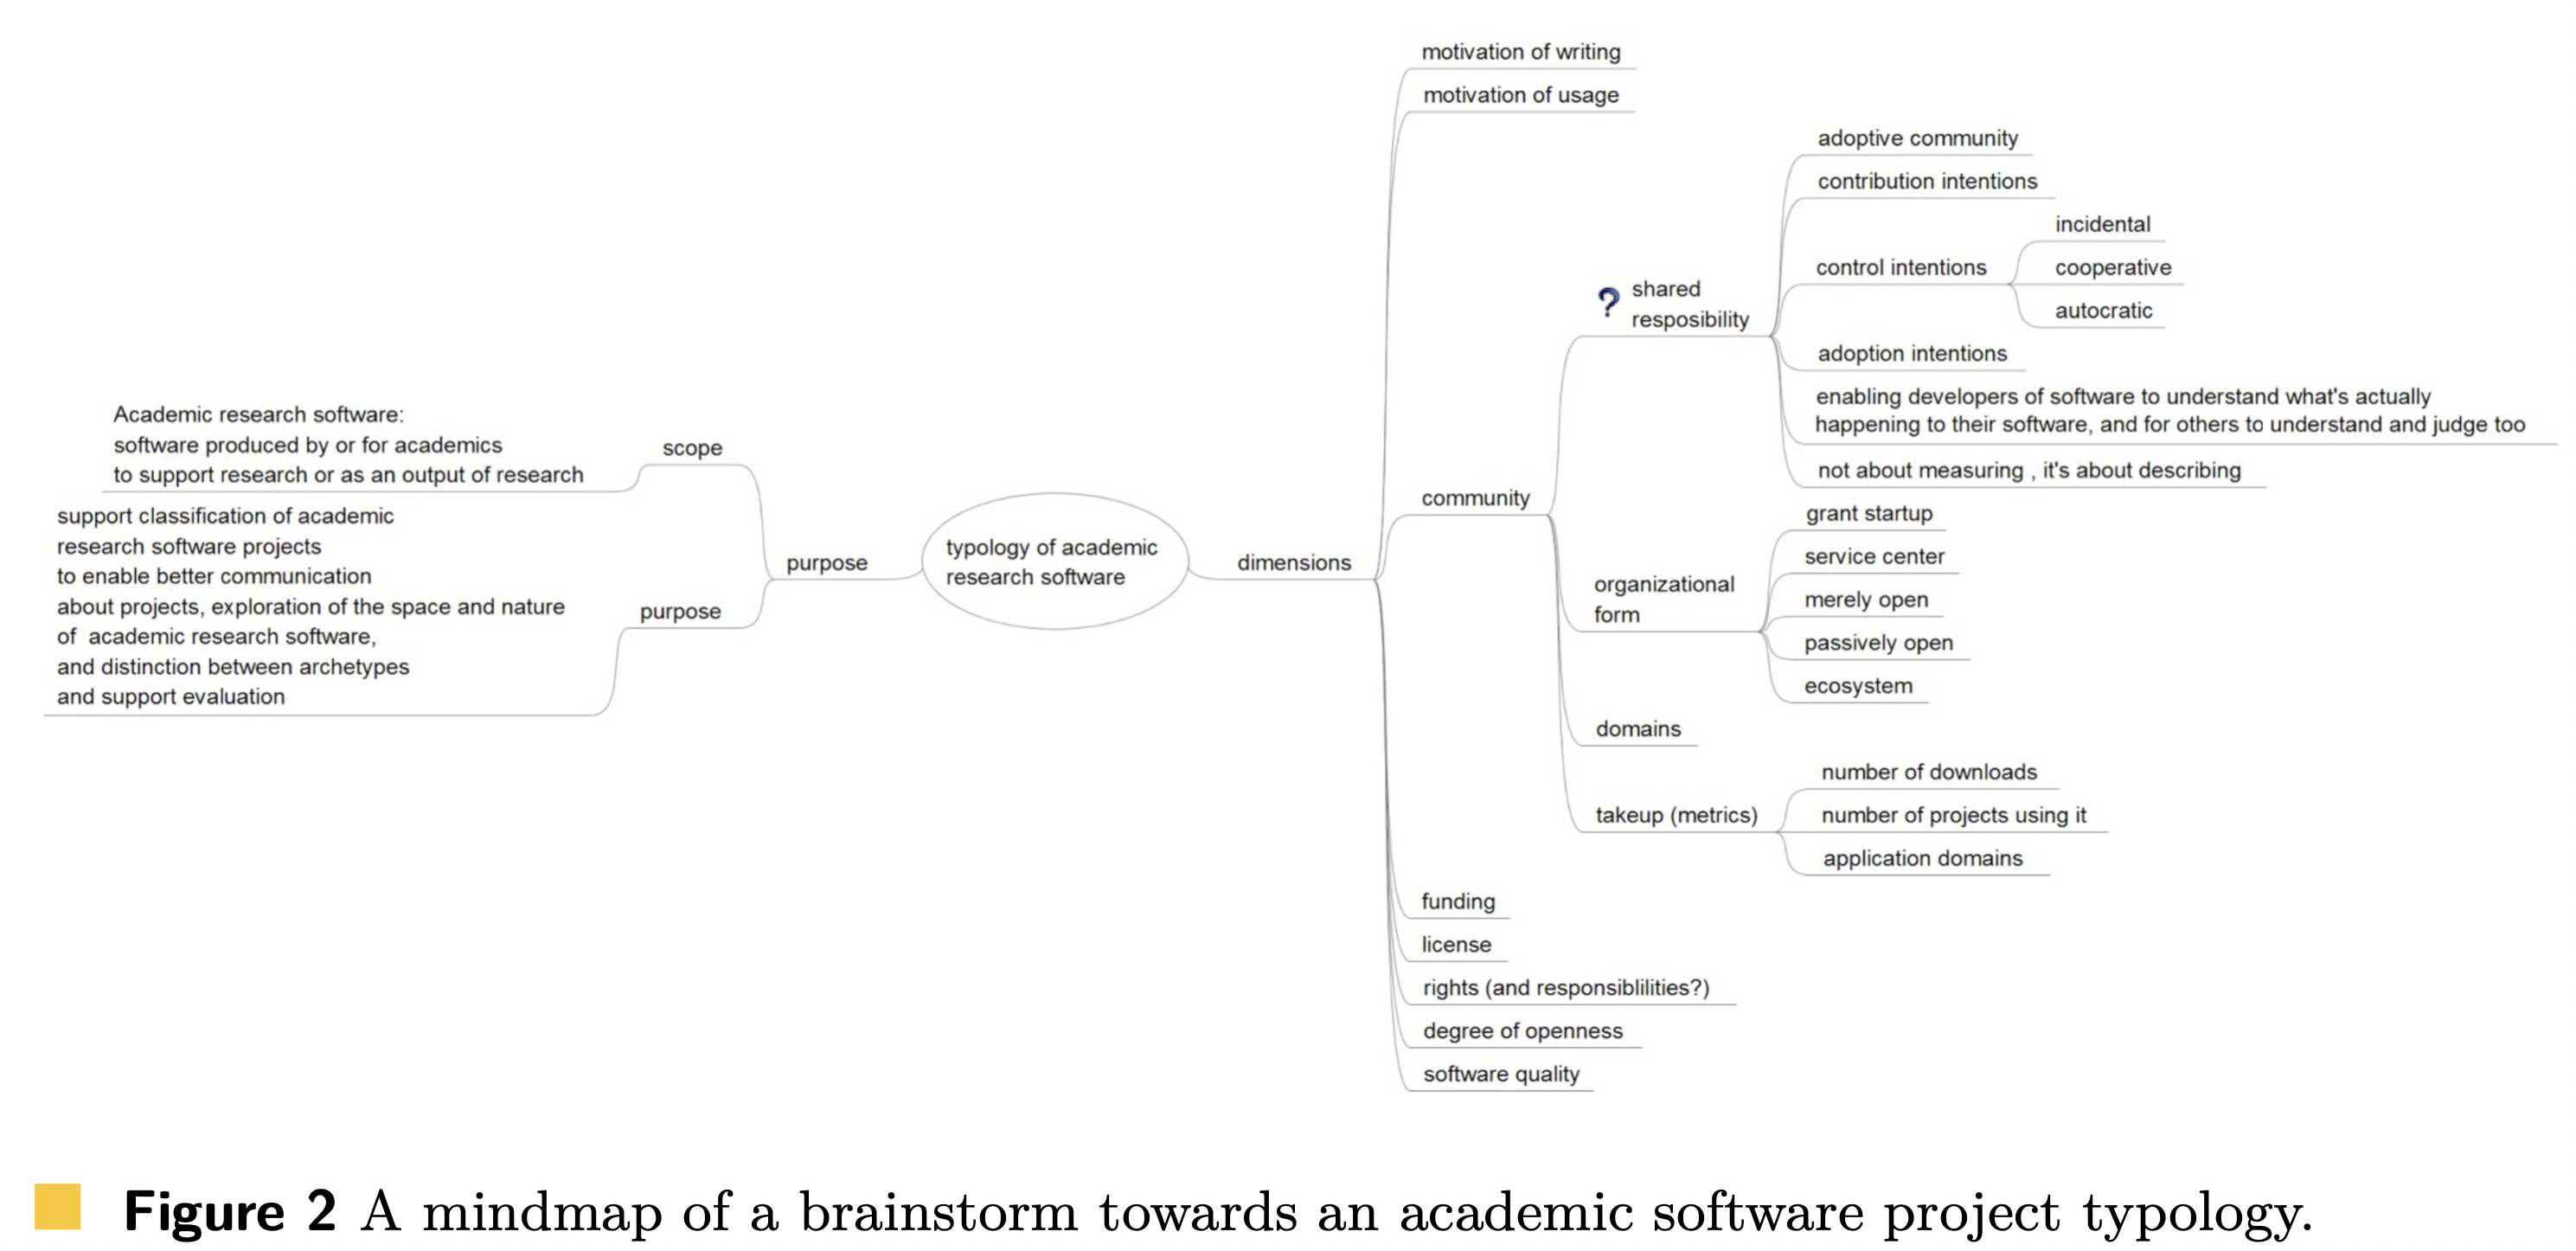
\includegraphics[scale=0.28]{JAI 2023/figures/RS-typology.png}
%    \caption{Figura do mindmap -- ontologia [CITAR]}
%    \label{fig:mindmap}
%\end{figure}
%
Como produto de software, o \RSw deve considerar alguns atributos de qualidade desejáveis.
%, sob diferentes perspectivas, por exemplo, usuários, desenvolvedores, e outros interessados. 
Por exemplo, é desejável que o \RSw seja confiável, eficiente, fácil de usar, fácil compreender, testar, reparar, estender ou adaptar.
%Podemos considerar que tais atributos podem estar associados ao software ou ao seu processo de desenvolvimento.
% 
Em especial, há uma preocupação com a sustentabilidade do \RSw e sua influência na reprodutibilidade da pesquisa científica.

Neste capítulo, apresentamos aspectos relacionados à  sustentabilidade do \RSw e boas práticas para o desenvolvimento de software sustentável, a saber: 
registro e identificação do software, licenças de software e grau de abertura (\textit{openness}), reconhecimento e citação do software, comunidade e usuários, longevidade e manutenibilidade, aderência aos princípios FAIR para software, avaliação do \RS e sua influência na reprodutibilidade científica.

%All research software is open
%All research software is high-quality and robust
%All research software is findable, accessible, and usable & used by others (for their own research), and is cited when it is used
%All contributors to research software are recognized for their work, with good careers
%All research software is sustained as long as it is useful
%All research is reproducible

%--------------------------------------------% 
\subsection{Sustentabilidade}
\label{subsection:srs}
%--------------------------------------------% 

% O desenvolvimento sustentável atende às necessidades do presente sem comprometer a capacidade das gerações futuras de atender às suas próprias necessidades. O desenvolvimento sustentável exige esforços conjuntos para a construção de um futuro inclusivo, sustentável e resiliente para as pessoas e o planeta.

\textit{Sustentabilidade} é um dos princípios norteadores da Ciência Aberta~\cite{unesco:2021} e define que a mesma
deve se basear em práticas, serviços, infraestruturas e modelos de financiamento de longo prazo que garantam a participação igualitária dos indivíduos que produzem ciência originários de instituições e países menos privilegiados. 
As infraestruturas científicas abertas devem ser organizadas e financiadas com base em uma visão essencialmente sem fins lucrativos e de longo prazo, que aprimorem as práticas de Ciência Aberta e garantam o acesso permanente e irrestrito a todos, na medida do possível.
%
No contexto da Ciência Aberta e sua dependência 
no código aberto (Seção~3.2.5), observa-se uma preocupação crescente com a sustentabilidade do software usado ou desenvolvido durante a pesquisa, em especial, com a longevidade e disponibilidade do software, e seu impacto na reprodutibilidade científica.
%

% Desenvolvimento sustentável, definido pela Comissão Brundtland [Brundtland, 1997] trata de "satisfazer as necessidades do presente sem comprometer a capacidade das gerações futuras de atender às suas próprias necessidades".

O tema Sustentabilidade, inicialmente associado ao campo da Ecologia, agora faz parte dos interesses de outras áreas do conhecimento, ainda que adaptado às especificidades de cada uma. 
Na Ciência da Computação, a preocupação com a sustentabilidade emerge como um tópico importante em diversas subáreas, incluindo Inteligência Artificial, Computação de Alto Desempenho, Interação Humano-Computador, Computação Científica e Engenharia de Software \cite{venters_software_2021}.
Sustentabilidade é um desafio a ser enfrentado, não um problema a ser resolvido~\cite{becker_2014}.

O \textit{Manifesto de Karlskrona} para o Design Sustentável~\cite{becker_2014}
define que sustentabilidade é, em sua essência, um conceito sistêmico, multi-facetado e deve ser entendida em um conjunto de cinco dimensões:
recursos ambientais, social, bem-estar individual, prosperidade econômica e viabilidade técnica de longo prazo.

Neste capítulo, abordamos aspectos da dimensão técnica da sustentabilidade do
software~\cite{DBLP:conf/re/KehrerP18} e, de forma complementar, elementos de sua dimensão social~\cite{DBLP:journals/sigsoft/Souza23}. 
% ou questões sócio-técnicas, e 
Não trataremos de aspectos da Engenharia de Software Verde~\cite{ivan:green:2018}\footnote{A Engenharia de Software Verde leva em consideração práticas e arquitetura de software, design de hardware e \textit{data center}, o mercado de eletricidade e mudanças climáticas, visando gerar menos emissões de gases de efeito estufa e reduzir produção de carbono de uma empresa~\cite{ivan:green:2018}.}.

\subsection*{Sustentabilidade de Software}
\label{subsection:sustainability}

Na Engenharia de Software, há duas linhas de pesquisa voltadas para Sustentabilidade que se destacam: 
(i)~Sustentabilidade de Software, e 
(ii)~Engenharia de Software para Sustentabilidade (SE4S). 
%
A pesquisa sobre \textit{Sustentabilidade de Software} tem como preocupação central a capacidade do software de perdurar ao longo do tempo,
enquanto que a pesquisa relacionada a SE4S preocupa-se com
sistemas intensivos em software, como integrar a sustentabilidade em seus processos de desenvolvimento de software
e apoiar a sustentabilidade ambiental
na ampla variedade de domínios em que o software é implantado \cite{venters_software_2021}.
%
%Entre estes dois universos há ainda um grande espaço para debate e construção de um entendimento comum sobre os conceitos fundamentais de sustentabilidade e como ela se relaciona com o software, visto que não há um acordo na comunidade de software sobre a definição de sustentabilidade de software ou como ela deve ser atingida. Apesar das inúmeras contribuições para formalizar a definicao de sustentabilidade de software, o conceito continua intangível e ambíguo, com indivíduos, grupos e organizacional mantendo visões diametralmente opostas.

No que se refere à sustentabilidade de software,
a longevidade como expressão de tempo (``longo prazo'') e a capacidade de manutenção são fatores-chave para sua compreensão~\cite{venters_2018}.
%
A preocupação com a longevidade do software estende-se ao atributo de manutenibilidade, e ao modelo e processo de desenvolvimento de software adotados, que podem influenciar atributos relacionados à sustentabilidade.
A manutenibilidade é reconhecidamente uma qualidade interna fundamental de sistemas de software~\cite{iec2014iso}, 
enquanto que a sua relação com a sustentabilidade de software ainda é objeto de pesquisa na área.
%
O termo sustentabilidade propriamente dito ainda não está bem definido neste contexto, deixando espaço para diferentes interpretações, e ainda há pouca evidência ou orientação sobre processos ou modelos de desenvolvimento voltados para a sustentabilidade de software~\cite{venters_software_2021}.
%Assim, definir sustentabilidade de software como a capacidade de perdurar ou como mais uma qualidade de software ao lado de manutenibilidade ainda não se mostra suficiente.

% The relationship between software quality and software sustainability is still an open question.
De um ponto de vista puramente técnico, \cite{venters_software_2021} define sustentabilidade de software como um requisito composto, não-funcional, de primeira classe, abrangendo as medidas de alguns conceitos centrais de atributos de qualidade de software, incluindo, no mínimo, manutenibilidade, extensibilidade e usabilidade.
Na dimensão técnica, a sustentabilidade de software está relacionada às consequências de longo prazo de projetar, construir e entregar um projeto de software e se espalha por diversas áreas, dentre elas, qualidade de software e métricas, requisitos de software e arquitetura de software~\cite{DBLP:conf/re/KehrerP18,venters_software_2021}.
Por fim, sustentabilidade de software diz respeito a assegurar que o software continue funcional para seus usuários ao longo do tempo, considerando também sua manutenção, inclusão de novos recursos, reparo de \textit{bugs}, e adaptações a novos ambientes de software e hardware.

%Portanto uma possivel abordagem para definir sustentabilidade de software eh como uma medida dos atributos: manutenibilidade, extensibilidade e usabilidade.

%In the case of software this means that it must continue to be available in the future, on new platforms and meeting new needs.
%How can we ensure sustainability of scientific software? What does this mean for a particular project?

\subsection*{Software de Pesquisa Sustentável}

O \textit{Software de Pesquisa Sustentável} deve permanecer \textit{disponível e funcional} para a comunidade científica durante períodos de tempo significativos. 
Não há uma resposta geral para a questão de quanto tempo o software precisa ser sustentado ou mantido. Este período pode depender da área de pesquisa, finalidade, função, frequência de uso, e da comunidade que o desenvolveu.

Sustentabilidade de \RSw inclui o processo de desenvolvimento e manutenção de software para que o mesmo continue a cumprir seu propósito ao longo do tempo. 
%
Certamente, o \RSw sustentável precisará ser atualizado com novas funcionalidades e correções de \textit{bugs}, adaptado a novos ambientes computacionais, manter-se amigável aos seus usuários, tornar-se multiplataforma, ser testado e certificado.
Garantir que o \RSw continue executável é desafiador, sendo  mais trabalhoso e caro do que um arquivamento simples de uma versão do software.  
As alterações necessárias para que o software permaneça executável devem garantir a confiabilidade nos resultados gerados pelas versões mais antigas do software. 
Se os resultados forem diferentes, justificativas objetivas devem ser fornecidas. 

Há diversas maneiras de promover e investir na sustentabilidade do \RS, incluindo atração de desenvolvedores, suporte à comunidade de usuários, busca por financiamento ou até comercialização -- todas válidas, desde que resultem na disponibilidade de longo prazo do software para a comunidade científica. 
Espera-se que, por meio da publicação de instruções, diretrizes e outras formas de ajuda e suporte, pesquisadores sejam capazes de decidir a forma de manter o seu software sustentável.

% Sustainable software engineering (SSE)

% Sustainable software engineering [4] motive is to create reliable, lifelong software that meets the needs of user’s requirement and also tried to reducing ecological impacts; its aim is to generate better software so there is no need to compromise future generations’ opportunities.

\subsection{\textit{FAIRness}}
\label{subsection:fair:software}

%Computational research should be FAIR: Findable, Accessible, Interoperable, Reusable. [CITAR algo]
% A modified version of these principles can be usefully applied to software too:  it should be Findable, Accessible, Reusable and Extensible. [Software as Output]

Os princípios FAIR~\cite{Wilkinson2016} foram especificados para melhorar o reuso de dados de pesquisa digitais, tornando-os mais fáceis de encontrar, acessíveis, interoperáveis e reutilizáveis (\textbf{F}indable, \textbf{A}ccessible, \textbf{I}nteroperable, \textbf{R}eusable).
%
Tais princípios abordam a \textit{forma} de fornecer artefatos para a comunidade científica, mas não tratam do conteúdo funcional ou da qualidade dos artefatos~\cite{lamprecht:2020}.
%\textbf{F}indability, \textbf{A}ccessibility, \textbf{I}nteroperability, \textbf{R}eusability.
Os \textit{Princípios FAIR para Dados de Pesquisa}~\cite{Wilkinson2016}, 
incluindo quatro princípios fundamentais e 15 princípios norteadores, estabelecem que os dados de pesquisa devem ser facilmente localizáveis, acessíveis, interoperáveis e reutilizáveis. 

Segundo~\cite{chue_hong_fair_2022}, o \RSw deve seguir os princípios FAIR usados para dados abertos, considerando-se que
o software também é um artefato de pesquisa digital e, como tal, deve ser facilmente localizável, acessível, interoperável e reutilizável. 
%
Os \textit{Princípios FAIR para Software de Pesquisa} (FAIR4RS) foram definidos a partir de uma reformulação dos princípios FAIR originais para dados abertos~\cite{lamprecht:2020,chue_hong_fair_2022,barker:2022}.
É importante destacar que, diferentemente dos dados, o software não é um artefato estático e só pode ser (re)utilizado se for sustentável~\cite{lamprecht:2020}.
%
A Tabela~\ref{tab:fairness:4:rs:r} apresenta a versão mais recente dos princípios FAIR para \RS.

\textit{Projetos de Software Livre} seguem os princípios FAIR. %recomendados para \RS.
Software livre pode ser localizado em repositórios com base em identificadores e descritores, utilizando diversos critérios como palavras-chave, linguagem de programação, versão do software, entre outros. 
A acessibilidade é encorajada em software disponível em repositórios abertos, com licenças de compartilhamento explícitas e bem definidas e documentação associada. 
A definição de interfaces de programação, formatos de entrada/saída e uso de padrões promovem a interoperabilidade e o reúso por vários grupos de pesquisa.
Nessa perspectiva, as práticas usadas no modelo de desenvolvimento de software livre podem ser adotadas no desenvolvimento e evolução de \RS~\cite{flach:sbc:2021}. 
%\footnote{\url{https://www.sbc.org.br/component/flippingbook/book/53/1?page=1}}

% Fairness template
\begin{table}[htbp]
    \caption{Princípios FAIR para Software~\cite{barker:2022}.}
    \centering
    \small
    \begin{tabular}{p{1.1cm}|p{13cm}}
    \hline
    \textbf{Princ.} & \textbf{Descrição} \\ \hline
    F: & Software, and its associated metadata, is easy for both humans and machines to find.\\
    F1 & Software is assigned a globally unique and persistent identifier.\\
    F1.1 & Software components representing granularity levels are assigned distinct identifiers.\\
    F1.2 & Different versions of the software are assigned distinct identifiers.\\
    F2 & Software is described with rich metadata. \\
    F3 & Metadata clearly and explicitly include the identifier of the software they describe.\\
    F4 & Metadata are FAIR, searchable and indexable.\\ \hline
    A: & Software, and its metadata, is retrievable via standardised protocols.\\
    A1 & Software is retrievable by its identifier using a standardised communications protocol. \\
    A1.1 & The protocol is open, free, and universally implementable.\\
    A1.2 & The protocol allows for authentication and authorization procedure, where necessary. \\
    A2 & Metadata are accessible, even when the software is no longer available.\\ \hline
    %\textbf{Princ.} & \textbf{Descrição} \\ \hline
    I: & Software interoperates with other software by exchanging data and/or metadata, and/or through interaction via application programming interfaces (APIs), described through standards.\\
    I1 &  Software reads, writes and exchanges data in a way that meets domain-relevant community standards.\\
    I2 & Software includes qualified references to other objects.\\
      \hline
    R: & Software is both usable (can be executed) and reusable (can be understood, modified, built upon, or incorporated into other software).\\
    R1 & Software is described with a plurality of accurate and relevant attributes.\\
    R1.1 & Software is given a clear and accessible license. \\ 
    R1.2 & Software is associated with detailed provenance.\\
    R2 & Software includes qualified references to other software.\\
    R3 & Software meets domain-relevant community standards. \\
      \hline
    \end{tabular} \label{tab:fairness:4:rs:r}
\end{table}

%Lots of work beyond FAIR: quality, correctness, reproducibility, openness, ...

%---------------------------------------------%
%Possivel referencia para avaliar se inclui ou nao: https://www.youtube.com/watch?v=67Uc1EEVDv8&t=953s

%O uso de \textit{Software de Pesquisa} é mencionado na literatura por meio de citação formal ou informal~ \cite{smith2016software} e está estreitamente relacionado ao sistema econômico de reputação científica, uma vez que tais menções causam impacto científico direto tanto na publicação quanto no ecossistema de software de pesquisa \cite{katz2014transitive}.

%Conhecimento novo é claramente construído a partir do conhecimento passado e o sistema de citações formais tem promovido avanços significativos \cite{katz2014transitive}.
% No entanto, isso não tem funcionado tão bem para produtos digitais como o software que, muitas vezes, dependem de outro software, fragmentos de código, e algoritmos \cite{katz2014transitive}.


\begin{comment}
\begin{table}[btp]
\begin{tcolorbox}[colback=white,title=Princípios FAIR para Software]
  \begin{description}
    \item \textbf{Localizável} \textit{(\textbf{F}indable)}
    
        O Software possui um rico conjunto de metadados e um identificador único e persistente que facilita sua busca e identificação.
    \item \textbf{Acessível} \textit{(\textbf{A}ccessible)}
    
        Os metadados do Software estão organizados e especificados em um formato legível para pessoas e máquinas. O Software e metadados devem estar depositados em repositórios públicos e reconhecidos pela comunidade.
    \item \textbf{Interoperável} \textit{(\textbf{I}nteroperable)}
    
        O Software usa padrões e plataformas reconhecidos pela comunidade possibilitando a integração com outras ferramentas e sistemas.
    \item \textbf{Reutilizável} \textit{(\textbf{R}eusable)}
    
        O Software possui uma licença e documentação que permitem sua adoção e extensão por outros pesquisadores e desenvolvedores. 
    \end{description}
\end{tcolorbox}
\end{table}
\end{comment}

%-----------------------------%
\subsection{Reprodutibilidade} \label{subsection:srrs}

A \textit{Reprodutibilidade} é um dos fundamentos do método científico e um princípio norteador da Ciência Aberta~\cite{unesco:2021}.
A boa prática científica exige que os artefatos de pesquisa mencionados em publicações científicas sejam mantidos e fiquem disponíveis para escrutínio dos pares, reprodução independente e verificação de resultados.

%Qual a importância da sustentabilidade do \RS para a pesquisa reprodutível aberta?  
%Lançamentos.
Para o \RS, a submissão ou publicação de um artigo é um dos momentos em que a versão do software usada no estudo precisa ser identificada, documentada e lançada.
% 
Se houver modificações no \RS, elas precisam ser registradas, 
usando algum esquema de nomenclatura que identifique o 
\textit{<software>}, a \textit{<versão>} e o \textit{<lançamento>}.
Em geral, a versão refere-se a mudança estratégica durante a evolução do software e o lançamento refere-se a mudanças simples de serviço.

A recomendação para que pesquisadores compartilhem e permitam o acesso aos dados descritos em suas publicações científicas, não garante a reprodutibilidade da pesquisa. 
Na prática, pesquisadores devem compartilhar o código de todo o \RSw desenvolvido e fluxos de trabalho de suas pesquisas para assegurar a reprodutibilidade.
Na maioria dos casos, o arquivamento de baixo custo do software, acompanhado de documentação clara deve ser suficiente.

Diretrizes para o desenvolvimento sustentável de \RSw também podem contribuir para a condução de uma pesquisa científica reprodutível,
apresentando princípios e boas práticas da engenharia de software.
As implementações das diretrizes podem variar entre os diferentes domínios científicos, mas as implementações devem ser públicas, abertas para discussão entre os pesquisadores e continuamente adaptadas em reposta às mudanças tecnológicas e nos domínios.

%In most cases, cheap software archiving with clear documentation (including version control, etc.) should be sufficient. 
% For this aspect of software sustainability, it is urgently needed that guidelines are given to all researchers, in particular those that are still in a phase before the actual conception of new software, on coding ethics, good practices, and other guidelines to make later use easier, once the software or tools have been created. 


%---------------------------------%
\subsection{Avaliação de \RS}

Consideramos a avaliação do \RSw sob duas perspectivas: (1)~sustentabilidade ou direcionada a sua longevidade, e (2)~aderência aos princípios FAIR (\textit{FAIRness}) ou direcionada ao grau de abertura (\textit{openness}) do \RS.

%Os princípios FAIR são critérios de referência para promover e avaliar a abertura (\textit{openness}) dos dados e do software de pesquisa.

\subsection*{Sustentabilidade}

A avaliação da sustentabilidade do \RSw busca determinar se o mesmo é sustentável com base em critérios relevantes para o ecossistema científico.
Em geral, a avaliação não gera um resultado \textit{é sustentável/não é sustentável}, mas tende a 
valorizar pontos fortes do software e identificar pontos para sua melhoria. A avaliação pode considerar atributos ou práticas usadas no desenvolvimento do software para 
prover uma visão geral ou detalhada da sustentabilidade do \RS.

O Instituto de Sustentabilidade de Software (SSI)
fornece um serviço de avaliação quantitativa do software baseada em critérios relacionados a sustentabilidade, manutenibilidade e usabilidade\footnote{
O questionário do SSI para avaliação de sustentabilidade está disponível em \url{http://www.software.ac.uk/online-sustainability-evaluation.}}.
%
A avaliação é feita com base em respostas dadas a um conjunto
de perguntas simples, seguidas por explicações sobre a importância de algumas práticas e recomendações. 
O conjunto de perguntas é aplicável para \RS.

Por exemplo, para uma resposta negativa para a pergunta 
``\textit{Seu \RSw está disponível como um pacote que pode ser instalado sem compilar?}'', a avaliação oferece a recomendação geral 
``Construir software pode ser complicado e demorado. Fornecer seu \RSw como um pacote que pode ser implantado sem compilar pode economizar tempo e esforço dos usuários, especialmente se não forem desenvolvedores de software. Idealmente, deve-se observar e testar se o \RSw é compilado e executado em diversas plataformas para as quais ele oferece suporte, para então prover pacotes para sua distribuição.'' 
%, o que significa que você já terá criado pacotes que podem ser distribuídos para seus usuários.

% \textit{Seu site e documentação fornecem uma visão geral clara e de alto nível do seu software?}, \textit{Seu software está disponível como um pacote que pode ser instalado sem compilar?}, \textit{Você publica seu histórico de lançamentos, por exemplo, dados de lançamento, números de versão, principais recursos de cada lançamento, etc., em seu site ou em sua documentação?},  \textit{Você tem um conjunto de testes automatizados para seu software?} ou \textit{Há uma citação recomendada para seu software?}.

Em nossa pesquisa, a avaliação de sustentabilidade  é simples, baseada em práticas, e busca determinar se um \RSw foi desenvolvido seguindo boas práticas que potencialmente o qualificariam como software sustentável. As práticas usadas em nossas avaliações estão relacionadas a identidade e disponibilidade do software, adoção de licenças, controle de versão, documentação, estrutura do código-fonte, testes, política de contribuidores e suporte, entre outras. 
O resultado de cada avaliação é sintetizado em uma tabela
e apresentado em um relatório simples.
%
A Tabela~\ref{tab:ssi:criteria:template} mostra práticas e aspectos que consideramos na avaliação da sustentabilidade 
de \RS.
%e do eventual desenvolvimento de novo software para substituí-lo. 
%--- criteria template ---%
\begin{table}[tbp]
    \caption{Avaliação de sustentabilidade do \RSw baseada em práticas.}
    \centering
    \small
    \begin{tabular}{p{0.65cm}|p{9cm}|c|p{2cm}}
    \hline
       \textbf{P} & \textbf{Descrição} & \textbf{Atende?} & \textbf{Comentário}\\
       \hline
        P1 & O software está hospedado em um repositório público  &  &  \\
        P2 & O software utiliza controle de versão  &  & \\
        P3 & O software adota explicitamente uma licença  &  & \\
        P4 & O software está registrado e apresenta um DOI &  &  \\
        P5 & A estrutura de arquivos do projeto de software comunica a finalidade de seus elementos &  & \\
        P6 & O software usa formato de dados e interfaces padronizadas  &  & \\
        P7 & A documentação apresenta uma visão geral do software &  &  \\
        P8 & O software possui testes &  &  \\
        P9 & O código é revisado antes de ser publicado  &  &  \\
        P10 & O projeto de software utiliza rastreador de tarefas e \textit{bugs}  &  &  \\
        P11 & Tarefas repetitivas são automatizadas  &  & \\
        P12 & Há integração e implantação contínuas  &  & \\
        P13 & Há lançamento de versões do software &  & \\
        P14 & Há evidência de uma comunidade (presente ou futuro) &  &  \\ 
        P15 & O software é divulgado para a comunidade acadêmica  &  & \\
        P16 & Há uma forma recomendada para citação do software  &  & \\
    \hline
    \end{tabular}
    \label{tab:ssi:criteria:template}
\end{table}


\subsection*{\textit{FAIRness}}

A avaliação de \textit{FAIRness} do \RSw pode ser definida como um processo de avaliação do seu grau de aderência aos princípios FAIR adaptados para software.
É importante lembrar que os princípios FAIR não são prescritivos, mas buscam oferecer uma visão para melhorar o compartilhamento e a reutilização de dados ou software por pessoas e máquinas~\cite{Wilkinson2016,chue_hong_fair_2022}.
%
Ainda assim, a avaliação de \textit{FAIRness} para software pode servir para apoiar a decisão de usuários e desenvolvedores sobre uma eventual adoção do \RSw em seu projeto de pesquisa.

No estudo apresentado neste capítulo, consideramos a versão mais recente dos princípios FAIR para software~\cite{barker:2022}.






%A Tabela~\ref{tab:fairness:parcial} mostra a avaliação parcial de \textit{FAIRness} de um \RS~\cite{lamprecht:2020}.
%
\begin{table}[tbp]
    \caption{Avaliação parcial de FAIRness.}
    \centering
    \small
    \begin{tabular}{p{0.9cm}|p{5cm}|c|p{6cm}}
    \hline
    Princ. & Description & Meets? & Comments 
    \\ \hline
    F: & Software, and its associated metadata, is easy for both humans and machines to find. & & \\
     F1 & Software is assigned a globally unique and persistent identifier. & YES & Partially: It does not have a specific PID, but it can be easily found across different repositories and registries including version information. \\
     F1.1 & Components of the software representing levels of granularity are assigned distinct identifiers. & & \\
     ... & ... & & \\
     A1 & Software is retrievable by its identifier using a standardised communications protocol. & YES & \textit{Both software and metadata are accessible through HTTPS ..: [..].} \\
     ... & ... & & \\
     R1.1 & Software is given a clear and accessible license. & YES & 
     \textit{Software: GNU General Public License as published by the Free Software Foundation, either version 3 of the license or later versions.} \\
     ... & ... & & \\
      \hline
    \end{tabular} \label{tab:fairness:parcial}
\end{table}

%A sustainability assessment can be defined as the process of identifying, measuring, and evaluating the potential impacts of alternatives for sustainability (Devuyst, 2000). 

% Relevance analysis -- is sustainability relevant?
% Scoping analysis -- what are the extent/depth, procedures and tools for the assessment?
% Impact analysis -- what are the short- and long-term economic, environmental and social impacts?
%  Comparative analysis -- what are the major synergies, conflicts and trade-offs?
% Associative analysis -- what measures can be put in place to mitigate harmful impacts?
% Political analysis -- which path is the least-cost (economic, environmental and social) option?

% Sustainability assessments can be broadly defined as processes that “direct the planning and decision-making process toward achieving sustainable development” (Hacking and Guthrie, 2008). Alternatively, sustainability assessment may be defined as processes integrating natural and societal systems, addressing both local and global dimensions, and covering both short-term and long-term perspectives (Ness et al., 2007), or processes determining whether an initiative is sustainable or not (Pope et al., 2004), or an evaluation against a set of sustainability principles 
\begin{comment}
Planos de gerenciamento de dados e software podem ser úteis para
fornecer um mecanismo para avaliação em diferentes pontos de verificação. Por exemplo, o plano de gerenciamento de software (SMP) ELIXIR\footnote{\url{https://github.com/elixir-europe/smp}} foi criado com o objetivo de elevar a qualidade e sustentabilidade do \RS, produzindo, promovendo, medindo e adotando as melhores práticas aplicadas ao ciclo de vida do desenvolvimento de software~\cite{elixir:smp}.

O projeto \textit{FAIRsFAIR} desenvolveu uma ferramenta de avaliação chamada \textit{FAIR-Aware}\footnote{\url{https://fairaware.dans.knaw.nl}} para ajudar pesquisadores a entender e melhorar a aderência de sua pesquisa aos princípios FAIR.
\end{comment}
\begin{comment}
SMP

Ao desenvolver um software de pesquisa, é fácil focar apenas em objetivos e atividades, como colaborar com outros pesquisadores, escrever artigos, participar de conferências e solicitar financiamento. Juntas, as demandas da prática diária de pesquisa podem conspirar para impedir o planejamento adequado para o desenvolvimento de software de pesquisa.

Um Plano de Gerenciamento de Software (SMP) pode ajudá-lo a definir um conjunto de estruturas e objetivos para entender seu software de pesquisa, incluindo o que você vai desenvolver; para quem é o software (mesmo que seja apenas para você); como você entregará seu software aos usuários pretendidos; como isso os ajudará; e como você avaliará se isso os ajudou e contribuiu para a pesquisa da maneira que você pretendia. Um SMP também ajuda você a entender como você pode apoiar aqueles que desejam ou usam seu software de pesquisa; como seu software se relaciona com outros artefatos em seu ecossistema de pesquisa; e como você garantirá que seu software permaneça disponível além da vida útil de seu projeto atual.

\end{comment}
